\documentclass[a4paper,UTF8]{article}
\usepackage{ctex}
\usepackage[margin=1.25in]{geometry}
\usepackage{color}
\usepackage{graphicx}
\usepackage{amssymb}
\usepackage{amsmath}
\usepackage{amsthm}
\usepackage{enumerate}
\usepackage{bm}
\usepackage{hyperref}
\usepackage{epsfig}
\usepackage{color}
\usepackage{tcolorbox}
\usepackage{mdframed}
\usepackage{lipsum}
\usepackage{tikz}
\newmdtheoremenv{thm-box}{myThm}
\newmdtheoremenv{prop-box}{Proposition}
\newmdtheoremenv{def-box}{定义}

\setlength{\evensidemargin}{.25in}
\setlength{\textwidth}{6in}
\setlength{\topmargin}{-0.5in}
\setlength{\topmargin}{-0.5in}
% \setlength{\textheight}{9.5in}
%%%%%%%%%%%%%%%%%%此处用于设置页眉页脚%%%%%%%%%%%%%%%%%%
\usepackage{fancyhdr}                                
\usepackage{lastpage}                                           
\usepackage{layout}                                             
\footskip = 10pt 
\pagestyle{fancy}                    % 设置页眉                 
\lhead{2019年春季}                    
\chead{大数据综合实验}                                                
% \rhead{第\thepage/\pageref{LastPage}页} 
\rhead{Task2}                                                                                               
\cfoot{\thepage}                                                
\renewcommand{\headrulewidth}{1pt}  			%页眉线宽,设为0可以去页眉线
\setlength{\skip\footins}{0.5cm}    			%脚注与正文的距离           
\renewcommand{\footrulewidth}{0pt}  			%页脚线宽,设为0可以去页脚线

\makeatletter 									%设置双线页眉                                        
\def\headrule{{\if@fancyplain\let\headrulewidth\plainheadrulewidth\fi%
		\hrule\@height 1.0pt \@width\headwidth\vskip1pt	%上面线为1pt粗  
		\hrule\@height 0.5pt\@width\headwidth  			%下面0.5pt粗            
		\vskip-2\headrulewidth\vskip-1pt}      			%两条线的距离1pt        
	\vspace{6mm}}     								%双线与下面正文之间的垂直间距              
\makeatother  

%%%%%%%%%%%%%%%%%%%%%%%%%%%%%%%%%%%%%%%%%%%%%%
\numberwithin{equation}{section}
%\usepackage[thmmarks, amsmath, thref]{ntheorem}
\newtheorem{myThm}{myThm}
\newtheorem*{myDef}{Definition}
\newtheorem*{mySol}{Solution}
\newtheorem*{myProof}{Proof}
\newcommand{\indep}{\rotatebox[origin=c]{90}{$\models$}}
\newcommand*\diff{\mathop{}\!\mathrm{d}}

\usepackage{multirow}
\usepackage{amssymb}
% 添加首行缩进,两个字符
\usepackage{indentfirst}
\setlength{\parindent}{2em}
%algorithm
\usepackage{algorithm}
\usepackage{algpseudocode} 
\renewcommand{\algorithmicrequire}{\textbf{Input:}} % Use Input in the format of Algorithm
\renewcommand{\algorithmicensure}{\textbf{Output:}} % Use Output in the format of Algorithm

\begin{document}
	\title{大数据综合实验\\
		金庸的江湖}
	\author{161220017, 陈翔}
	\maketitle
	\section{任务4:基于人物关系图的 PageRank 计算}
	在本次任务中,我们需要利用上次任务中生成的人物关系图计算各个人物的PageRank值。PageRank算法是一个用来评估网页重要性或等级的算法,这里我们采用该算法的并行形式解决问题。
	\begin{enumerate}[ {(}1{)}]
		\item 任务分析:
		
		观察输入我们可以发现,本次任务与一般的网页排名任务相比至少有两处区别:
		\begin{itemize}
			\item 对于某个节点,其各个邻居的权重并不相等。
			\item 这是一个对称图,即若节点$u$对$v$有贡献,那么反之亦然。
		\end{itemize}
		基于这两点观察,我们首先将改动了PR值的计算公式\ref{eq:pr}:
		$$
			\label{eq:pr} PR(u)=\sum_{v \in B_u} PR(v) \times w(v,u)
		$$
		其中$w(v,u)$表示节点$u$在$v$中所占比重,且$\sum_{v \in B_u}w(u,v) = 1$。其次,由于第二点,我们无需担心排名泄露或者排名下沉的情况,因此不必引入随机浏览模型。
		
		\item 伪代码实现:
		
		算法\ref{alg:prit}给出了本次任务的主体——PageRankIter的实现。我们应迭代该算法多次以得到较为稳定的PR值。因此,我们需要保持输入格式与输出格式的一致以保证该算法是可迭代的,这要求我们在每个Mapper中传递原始的图结构信息。
		
		算法的第2行是从输入文件中读取一行,并将其转换成方便处理的结构。
		
		算法的第3到5行在循环地处理某个人物(称为主人)的所有邻居,单个邻居的格式为(String, Double),其中第一个元素为邻居的名字,第二个元素为邻居的权重。我们以邻居为键,以主人的名字和主人的PR值与邻居权重的乘积组成的pair为值,发送给Reducer。
		
		算法的第3到5行在迭代处理某个人物(称为主人)的所有邻居,单个邻居的格式为(String, Double),其中第一个元素为邻居的名字,第二个元素为邻居的权重。我们以邻居为键,以主人的名字和主人的PR值与邻居权重的乘积组成的pair为值,发送给Reducer。
		
		算法的第6行将原输入稍作改动又发送了出去,目的在于维持图结构,加标识符是为了防止与第4行发送的信息产生混淆。
		
		算法的第9行依然是将输入转换成易处理的形式,并且初始化当前键的PR值为0。
		
		算法的第10行到第16行在迭代处理该键对应的每个值。对于算法第4行发送的值,直接累加到当前键的PR值上即可;而对于第6行发送的信息,则将其作为后缀与当前键和累加完毕的PR值一起在第17行被写到文件中去即可。
		\begin{algorithm}[htb] 
			\caption{ PageRankIter } 
			\label{alg:prit} 
			\begin{algorithmic}[1] 
				\Require 
				归一化权重后的人物关系图
				\Ensure 
				各个人物的PR值
				\Function {Mapper}{} 
				\label{function:Map}  
				\State 将人物关系图中的一行进行分割,得到(String,Double,Array[String,Double])的形式,称其为(nameKey,keyPR,neighbors)
				\For{neighbor in neighbors}
				\State	Emit(neighbor.name, (nameKey, keyPR $\times$ neighbor.weight))
				\EndFor
				\State	Emit(nameKey, (标识符,neighbors))
				\EndFunction
				\Function {Reducer}{} 
				\label{function:Reduce}  
				\State 将Mapper中发来的某个键-值列表对(key,[value])进行分割,并初始化pr为0
				\For{v in [value]}
				\If{v.first == 标识符}
				\State neighbors = v.second
				\Else 
				\State pr += v.second
				\EndIf
				\EndFor
				\State	Write(key, pr, neighbors)
				\EndFunction
			\end{algorithmic} 
		\end{algorithm}	
		图\ref{fig:pageiter}为该任务迭代进行50次的结果的前10行。
		\begin{figure}
			\centering
			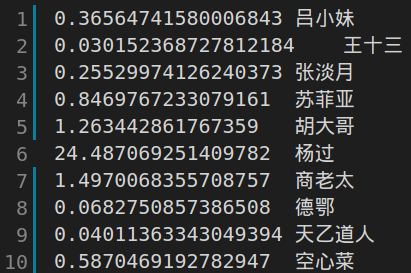
\includegraphics[width=0.7\linewidth]{graph/Task4PageIter}
			\caption[1]{PageRankIter运行50次}
			\label{fig:pageiter}
		\end{figure}
		\item 迭代文件:
		
		由于HDFS禁止覆盖已经存在的文件目录或文件,因此我们需要注意在主循环中的每次迭代中都要新建一个目录作为输出,再在下次迭代的时候将该输出作为输入。
		\item 输出优化(任务6选做):
		
		本任务中默认的输出是杂乱的。为了得到更直观的输出,我们还需实现一个排序算法PageViewer,使输出按降序,从而方便找到PR值最高几个人物。PageViewer实现很简单,我们只需要将任务4输出的key和value交换顺序重新输出即可,因为Mapreduce框架默认会对key值进行排序。需要注意的是,由于Mapreduce默认的排序方法是升序,因此我们需要重载比较器以实现降序,方法也很简单,返回原比较器的返回值的相反数即可。	
		图\ref{fig:pageviewer}为对原任务的输出进行了降序处理的前10行。
		\begin{figure}
			\centering
			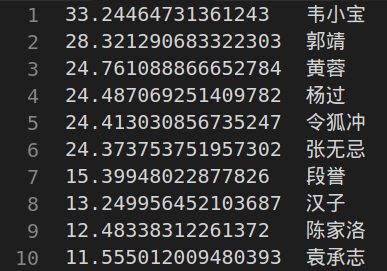
\includegraphics[width=0.7\linewidth]{graph/Task4PageViewer}
			\caption[2]{PageRankViewer运行结果}
			\label{fig:pageviewer}
		\end{figure}
		\item 运行截图:
		
		图\ref{fig:task4run}为本任务在集群上的运行时截图,其中命令最后的数字"1"表示迭代1次。
		\begin{figure}
			\centering
			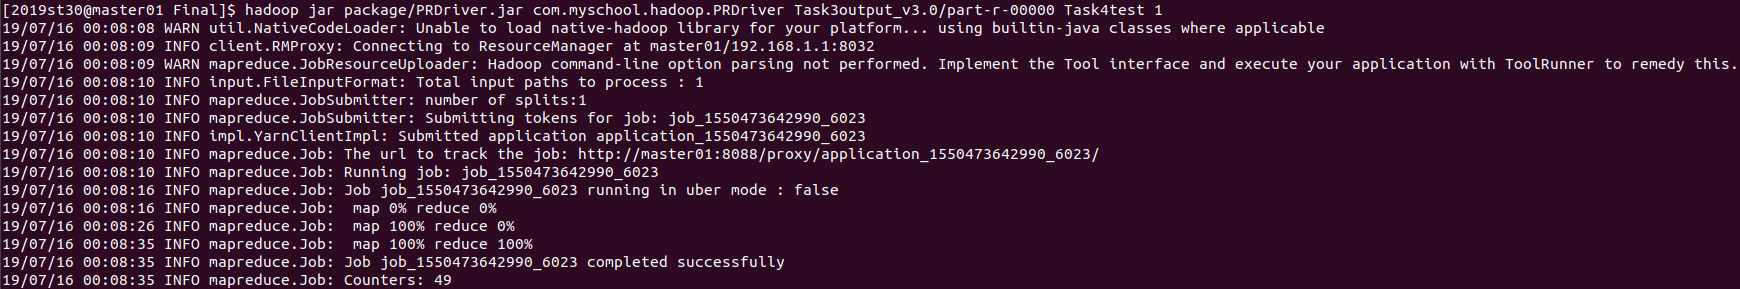
\includegraphics[width=0.7\linewidth]{graph/Task4Run}
			\caption[3]{任务4运行情况}
			\label{fig:task4run}
		\end{figure}				
		\item 性能分析:
		
		根据图\ref{fig:task4run}中map阶段与reduce阶段的速度,我们发现在本次实验的数据量下,迭代一次大约需要20秒,若再加上预处理和后续处理的时间,那么迭代一次需要27秒左右。若迭代50次,则大约需要22分钟。
		\item 收敛情况:
		\begin{figure}
			\centering
			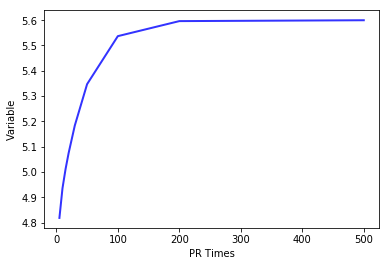
\includegraphics[width=0.7\linewidth]{graph/Task4PRTimes}
			\caption{迭代轮数/总体方差折线图}
			\label{fig:task4prtimes}
		\end{figure}
		
		根据图\ref{fig:task4prtimes},我们可以看出,随着迭代轮数的上升,PR值的方差不断上升,并且在迭代轮数超过200轮时趋于稳定。因此我们推荐将迭代轮数设置为200。
		
	\end{enumerate}		
	\section{附加部分:基于Spark的再实现}
	由于MapReduce框架最初是为高吞吐量的批量数据处理而设计的,因此并不擅长低延迟的情况,而本次实验的小数据量无疑放大了这一缺陷。同时,MapReduce框架还限制了操作为map、reduce等有限的几种类型,大大降低了编程的灵活性。因此,以内存计算为核心、集多种计算模式于一体的Spark框架是更加明智的选择。
	
	本次实验中,我们使用scala语言来编写spark程序,并且省略了预处理部分的再实现。
	\begin{enumerate}[ {(}1{)}]
		\item 人物同现算法:
		
		利用spark来实现人物同现算法相当容易,只需要短短的几行。
		
		首先我们需要读入文件并根据空格进行分割。注意到,读入文件的一行可能包含重复的人物,而根据预期结果我们去掉重复的。这两步在scala中只需要一行即可实现:		
		\begin{center}
		val words = spark.read.textFile(path).collect.map(line $=>$ line.split(" ").distinct)
		\end{center}
		需要注意的是,val表示变量是不变引用,这对于程序来说是较为安全的;相对地,var表示该变量是可变的。其中,collect是一个action操作,表示返回某个dataset的所有元素,在本语境中表示返回一个文件的所有行。map则是一个transformation操作,表示将每个元素转换为另外的元素,在本语境中,表示将每一行转换为每一行出现过的元素的集合。distinct也是一个transformation操作,返回一个dataset中不同的元素的集合。所有transformation操作都是惰性操作,只是定义了一个新的RDD,而并不马上计算新的RDD内部的值。而action操作都是立即操作,会立即计算新定义的RDD的值。
	
		其次,我们统计所有在一行中出现的人物对(包括逆对),实现如下:	
		\begin{center}
		val coTerm = words.map { line $=>$
			for{
				i $<-$ 0 until line.length
				j $<-$ (i+1) until line.length
			} yield {
				(line(i), line(j))
			} 
		}.flatMap(x $=>$ x).flatMap(x $=>$ List(x,(x.\_2,x.\_1)))
		\end{center}
		我们利用map操作遍历每一行中可能出现的所有人物对,并且通过flatMap将其合并到一起,最后再次利用flatMap将每个人物对的逆对也包含进去。其中,flatMap与map很像,也是一个transformation操作,区别在于后者将每个元素转换形成的元素集合进行了一次合并。
		
		最后我们将coTerm中相同的元素进行累加,实现如下:	
		\begin{center}
			val rdd = sc.parallelize(coTerm)
			val results = rdd.map(w $=>$ (w,1)).reduceByKey({case(x,y) $=>$ x+y})
		\end{center}
		第一行表示我们首先需要将coTerm转换为可并行化操作的数据结构,第二行则是一个简单的MapReduce过程,其中map将每一个人物对转换成了(人物对,1)的形式,reduceByKey则将人物对相同的键值对累加值并合并。
		
		图\ref{fig:stask2result},\ref{fig:stask4run}分别是该任务的运行结果和截图。
		\begin{figure}
			\centering
			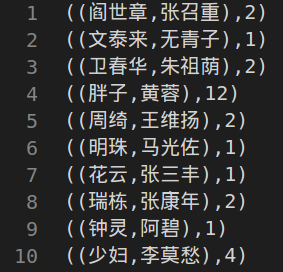
\includegraphics[width=0.7\linewidth]{graph/STask2Result}
			\caption[4]{任务2的Scala版本运行结果}
			\label{fig:stask2result}
		\end{figure}
		\begin{figure}
			\centering
			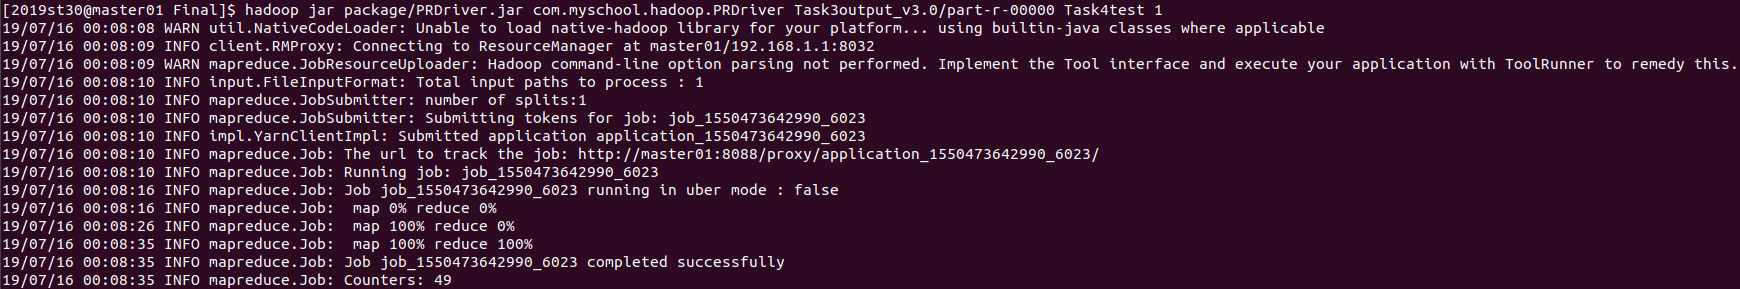
\includegraphics[width=0.7\linewidth]{graph/Task4Run}
			\caption[5]{任务2的Scala版本运行情况}
			\label{fig:stask4run}
		\end{figure}
		\item 人物关系图构建与特征归一化:
		
		我们可以利用两行代码来实现该任务:
		\begin{center}
			val sum = results.map(w $=>$ (w.\_1.\_1,w.\_2)).reduceByKey({case(x,y) $=>$ x+y}).collectAsMap()
			val weight = results.map(w $=>$ (w.\_1.\_1, (w.\_1.\_2, w.\_2.toDouble/sum(w.\_1.\_1)))).groupByKey()
		\end{center}
		在第一行,我们首先收集每个人物对应的所有邻居计数之和,并生成一个可供查询的字典。具体而言,我们把上一个任务中的每一个输出,例如((x,y),t),转换成(x,t)的形式,并再次利用reduceByKey合并并累加所有具有相同键的键值对。最后我们使用collectAsMap函数生成一个字典。
		
		在第二行,我们再次映射上一个任务中的输出,并将其转换为(x, (y, t/sum(x))的形式,其中sum(x)表示第一行生成的字典中x对应的值。然后我们再将每个键值对按key组合,生成(x, (y, [t/sum(x)])。
		\item 基于人物关系图的 PageRank 计算:
		
		我们的实现基于图\ref{fig:code}。
		\begin{figure}
			\centering
			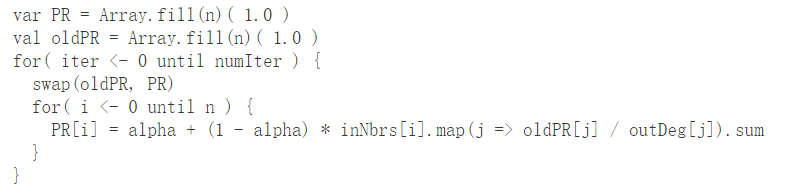
\includegraphics[width=0.7\linewidth]{graph/STask4Code}
			\caption[6]{spark手册实现样例}
			\label{fig:code}
		\end{figure}
		首先,我们需要将前一个任务生成的RDD转换为数组形式,以方便我们进行下标查询的操作。然后,我们需要对图\ref{fig:code}做些改动以得到适合本任务的算法,如下:
		\begin{center}
			var pr = Array.fill(n)( 1.0 )
			for( iter $<-$ 0 until times ) {
				var tmp = Array.fill(n)( 1.0 )
				val oldPR = pr
				for( i $<-$ 0 until n ) 
					tmp(i) = warray(i).\_2.map(j $=>$ oldPR(name2Idx(j.\_1))*weightOf(j.\_1,i)).sum
				pr = tmp
			}
		\end{center}
		具体而言,我们首先需要初始化数组pr,其中n是人物总数。为了令pr是可迭代的,我们需要将其类型设置为var。接着,我们在外层循环中迭代计算pr,其中变量tmp和oldPR是为了保证迭代的正确性,内层循环则刚好体现了\ref{eq:pr}的计算过程。其中,name2Idx(x)表示以x为键的键值对所对应的数组下标,weightOf(x,y)则表示下标y所对应的人物在x中所占比重。这两个函数都可通过遍历数组来实现。
		
		同样地,为了结果更加直观,我们需要对输出进行降序处理。令pair为(pr,x)键值对字典,我们只需要一行代码便可实现降序:
		\begin{center}
			val result = pair.sortBy(r $=>$ r.\_1)(Ordering.Double.reverse)
		\end{center}
		其中,sortBy函数指定了排序依据,在当前语境下即按pr值排序,第二个小括号内则规定了按降序还是升序。
		
		图\ref{fig:stask4runs}展示了scala版本的PageRank迭代50次开始时的情况,\ref{fig:stask4rune}则展示了运行结束时的情况。
		\begin{figure}
			\centering
			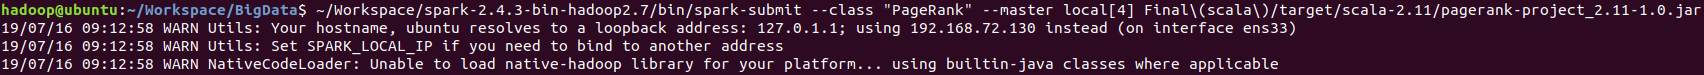
\includegraphics[width=0.7\linewidth]{graph/STask4RunS}
			\caption[7]{开始运行}
			\label{fig:stask4runs}
		\end{figure}
		\begin{figure}
			\centering
			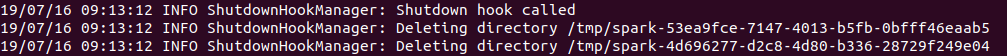
\includegraphics[width=0.7\linewidth]{graph/STask4RunE}
			\caption[8]{运行结束}
			\label{fig:stask4rune}
		\end{figure}
		
		据此我们可以得知scala版本的PageRank执行时间大约为14秒,相比于MapReduce版本的22分钟,快了将近100倍(\ref{fig:stask4runtime})。
		\begin{figure}
			\centering
			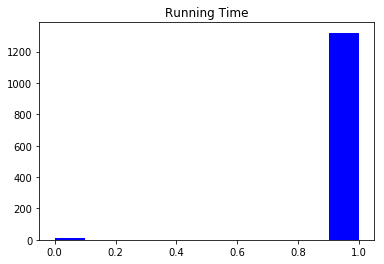
\includegraphics[width=0.7\linewidth]{graph/STask4RunTime}
			\caption[9]{运行时间对比(左边为scala)}
			\label{fig:stask4runtime}
		\end{figure}		
		
		图\ref{fig:stask4result}为本程序的运行结果,与MapReduce版本的结果几乎相同。
		\begin{figure}
			\centering
			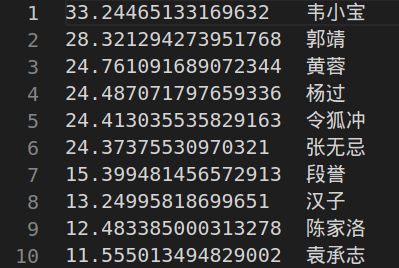
\includegraphics[width=0.7\linewidth]{graph/STask4Result}
			\caption[10]{运行结果}
			\label{fig:stask4result}
		\end{figure}
		
	\end{enumerate}

	\section{总结:实验过程中遇到的问题及解决办法}
	\begin{enumerate}[ {(}1{)}]
		\item 使用Java的split方法分割语句时,需要特别注意转义符“$\backslash$”的用法,比如当一行((line)按制表符分割时,我们需要使用line.split("$\backslash$$\backslash$t")来解析,而line.split("$\backslash$t")则会失败。
		\item 
		scala中的val表示引用的对象不变,但如果引用的对象为可变对象,则意味着val修饰的值也有改变的风险。例如
		\begin{center}
			var x = 1
			val y = x
		\end{center}
		表面上y是定值,我们也的确无法直接修改y的值变为2,但却可以通过修改x的值来间接地改变y。在编程中尤其要注意这点。
	\end{enumerate}
\end{document}